\chapter{电动力学}
\rightline{\it 电动力学是电的动力学,而不是电动的力学。}
\section{麦克斯韦方程组}
我们先来看看传说中的麦克斯韦方程组:
\begin{align*}
\nabla \cdot \mathbf{E}&=\frac{\rho}{\epsilon_0} & \nabla \cdot \mathbf{B}&=0 \\
\nabla \times \mathbf{E}&=-\frac{\partial \mathbf{B}}{\partial t} & \nabla \times \mathbf{B}&=\mu_0 \mathbf{j}+\frac{1}{c^2} \frac{\partial \mathbf{E}}{\partial t}
\end{align*}

这是麦克斯韦方程组在真空中的形式,没有考虑电磁介质。这些方程可以解出所有与电和磁有关的现象(如果不考虑量子效应),包括高中学过的库仑定律、楞茨定律等等,也包括电磁介质的性质。如果你第一次看到这些方程的时候一脸懵逼,连里面的三角形是什么意思都不知道,那也不用害怕,这一章我们会慢慢搞懂这些方程的意思。
\section{前两个麦克斯韦方程}
高中学过了点电荷周围的电场$E=k \frac{q}{r^2}$,如果以电荷为中心画一个半径为$r$的球面,$\mathbf{E}$的通量$\Phi=E \cdot 4 \pi r^2=4 \pi k q$。因为电场线是连续的,不管在外面画什么样的闭合曲面,上面的$\Phi$都是$4 \pi k q$。

如图\ref{fig-elec-flux},如果有许多电荷,曲面上的$\Phi$是曲面内各个电荷产生的$\Phi$之和;而曲面外的电荷产生的电场线在进入曲面之后肯定要出来,对$\Phi$没有影响。
\begin{figure}[htb]
\centering
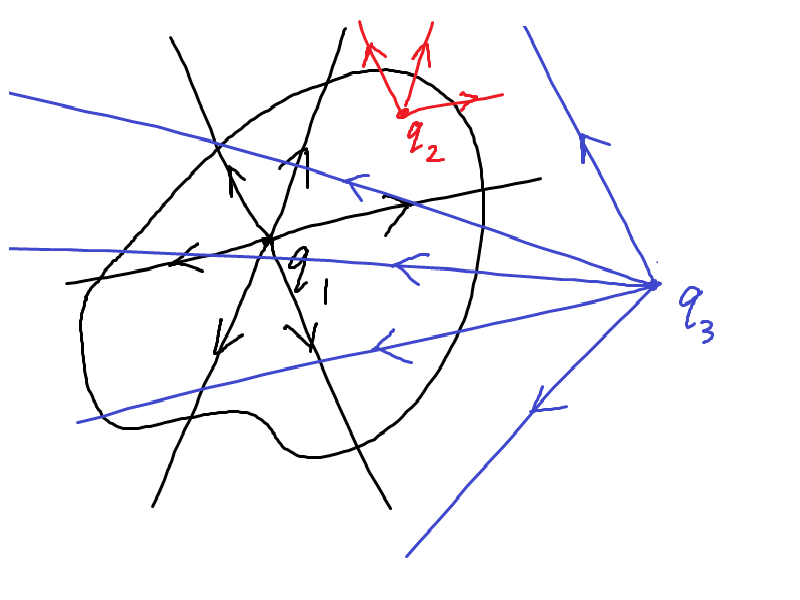
\includegraphics[scale=0.5]{fig/elec-flux}
\caption{里面和外面}
\label{fig-elec-flux}
\end{figure}

(这里分别画出了各个电荷产生的电场线,不用考虑它们的相互影响。电场线在某个点的方向就是这个点上$\mathbf{E}$的方向,我们经常看到两个电荷之间用弯曲的电场线连接,那是每个电荷产生的$\mathbf{E}$的矢量和。如果电场线从一个电荷开始,从另一个电荷终止,相当于这两个电荷的一条电场线相互抵消)

也就是说,$\Phi=4 \pi k \sum_V q_i$。在电动力学中会用另一个常量$\epsilon_0=\frac{1}{4 \pi k}$,称为真空介电常量,$\epsilon_0 \approx 8.85 \times 10^{-12} \unit{m^{-3} \cdot kg^{-1} \cdot s^4 \cdot A^2}$。如果把公式里的$k$换成$\epsilon_0$,就是$\Phi=\frac{1}{\epsilon_0} \sum_V q_i$。用$\epsilon_0$可以少写很多$4 \pi$。

按照高斯定理,$\Phi=\int_V \nabla \cdot \mathbf{E} \opd V$。这里有对$V$的积分,如果要把前面对$V$的求和改成积分,就要把电荷$q$改成电荷密度$\rho$:$\Phi=\frac{1}{\epsilon_0} \int_V \rho \opd V$。比较两个式子,可以发现$\nabla \cdot \mathbf{E}=\frac{\rho}{\epsilon_0}$。也就是说,第一个麦克斯韦方程对应着库仑定律或者电场的高斯定理。

(以后学了量纲分析之后,你可以检验一下它两边的量纲一样,注意$\nabla$的量纲是$[L]^{-1}$)

现在第二个麦克斯韦方程应该很好理解:$\nabla \cdot \mathbf{B}=0$表示磁感线是闭合的,不会变多变少,除非存在传说中的磁单极子。
\section{后两个麦克斯韦方程}
第三个麦克斯韦方程$\nabla \times \mathbf{E}=-\frac{\partial \mathbf{B}}{\partial t}$对应着法拉第电磁感应定律。按照斯托克斯定理,$\oint_L \mathbf{E} \cdot \opd \mathbf{L}=\int_S (\nabla \times \mathbf{E}) \cdot \opd \mathbf{S}$。而法拉第定律可以写成$\oint_L \mathbf{E} \cdot \opd \mathbf{L}=-\int_S \frac{\partial \mathbf{B}}{\partial t} \cdot \opd \mathbf{S}$,左边表示$L$上的感生电动势,右边表示$S$上磁通量的变化速率,负号表示感生电动势的方向按照楞茨定律确定。

第四个麦克斯韦方程的右边有两项。如果只有$\nabla \times \mathbf{B}=\mu_0 \mathbf{j}$,它表示电流在周围产生磁场。$\mathbf{j}$是电流密度,也就是单位面积上流过的电流,为了把面积上的求和改成积分,就要把$I$改成$\mathbf{j}$。$I$是标量,然而$\mathbf{j}$是矢量,$I$是$\mathbf{j}$的通量。你可以检验一下磁场方向与电流方向的关系确实是右手螺旋。

$\mu_0$是一个比例系数,叫作真空磁导率,$\mu_0=4 \pi \times 10^{-7} \unit{m \cdot kg \cdot s^{-2} \cdot A^{-2}}$。

第二项$\frac{1}{c^2} \frac{\partial \mathbf{E}}{\partial t}$又是什么意思呢?如图\ref{fig-disp-curr},有两根很粗的导线靠近但不接触,中间形成一个平行板电容器,两个极板分别是两根导线的末端。如果导线内没有电流,但是导线的末端积累着电荷,中间就有恒定的电场;如果导线内有电流,中间的电场就会变化。
\begin{figure}[htb]
\centering
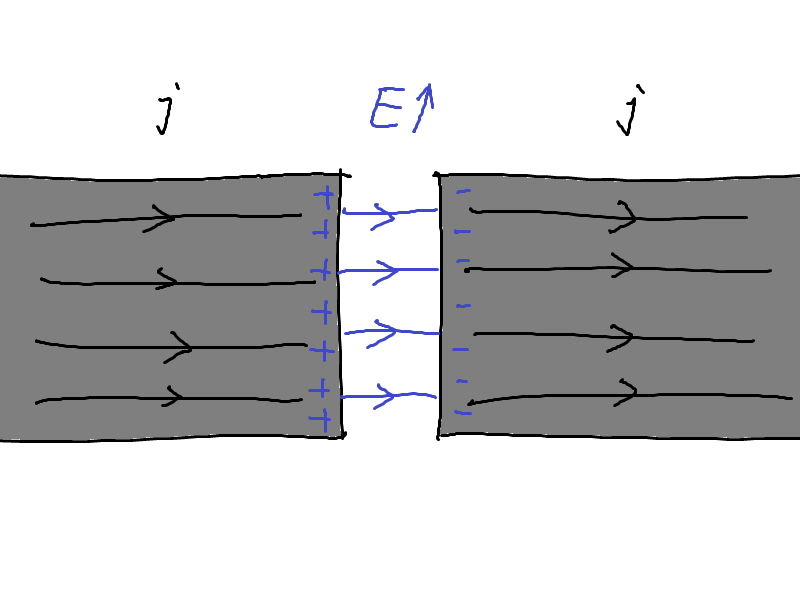
\includegraphics[scale=0.5]{fig/disp-curr}
\caption{位移电流}
\label{fig-disp-curr}
\end{figure}

电流会在周围产生磁场,所以麦克斯韦猜:变化的电场也会在周围产生磁场。所以他把变化变化的电流称为位移电流。准确地说,位移电流密度$\mathbf{j}_d=\epsilon_0 \frac{\partial \mathbf{E}}{\partial t}$,它的量纲与$\mathbf{j}$相同。

所以第四个麦克斯韦方程也可以写成$\nabla \times \mathbf{B}=\mu_0 (\mathbf{j}+\mathbf{j}_d)=\mu_0 \mathbf{j}+\epsilon_0 \mu_0 \frac{\partial \mathbf{E}}{\partial t}$。

我们可以定义另一个常数$c$,令$\epsilon_0 \mu_0=\frac{1}{c^2}$。$c$的量纲是速度,待会可以证明它是电磁波的速度。当时的人们用实验测出$\epsilon_0$和$\mu_0$,算出$c$,与其他方法测出的光速相同,所以麦克斯韦猜想光是一种电磁波。

$\frac{\partial \mathbf{E}}{\partial t}$前面的系数$\frac{1}{c^2}$非常小,所以从前一直没有被人们发现,直到麦克斯韦猜了出来,后来也得到了实验的证实。
\section{电磁波}
接下来我们用麦克斯韦方程组来算一些有意思的东西。既然变化的磁场在附近产生电场,变化的电场在附近产生磁场,那么它们可以不断产生并且向远处传播,即使在没有电荷和电流的\emph{自由空间}里也是一样。

在没有电流的情况下,$\nabla \times \mathbf{B}=\frac{1}{c^2} \frac{\partial \mathbf{E}}{\partial t}$。想办法让其他方程出现$\nabla \times \mathbf{B}$,可以对$\nabla \times \mathbf{E}=-\frac{\partial \mathbf{B}}{\partial t}$两边同时取旋度,得到$\nabla \times (\nabla \times \mathbf{E})=-\ppt(\nabla \times \mathbf{B})=-\frac{1}{c^2} \pptn{2} \mathbf{E}$。($\nabla \times$和$\ppt$可以交换顺序)

接着处理式子的左边,按照矢量分析的公式,$\nabla \times (\nabla \times \mathbf{E})=\nabla(\nabla \cdot \mathbf{E})-\nabla^2 \mathbf{E}$。在没有电荷的情况下,$\nabla \cdot \mathbf{E}=0$,剩下$-\nabla^2 \mathbf{E}$。

也就是说,$-\nabla^2 \mathbf{E}=-\frac{1}{c^2} \pptn{2} \mathbf{E}$,一般写成$\pptn{2} \mathbf{E}=c^2 \nabla^2 \mathbf{E}$,也就是$\pptn{2} \mathbf{E}=c^2 (\ppxn{2} \mathbf{E}+\ppyn{2} \mathbf{E}+\ppzn{2} \mathbf{E})$。简单起见,在一维情况下,$\pptn{2} \mathbf{E}=c^2 \ppxn{2} \mathbf{E}$,$\mathbf{E}$是$x,t$的函数。

如果把$\mathbf{E}$的某个分量记为$f$,它满足方程$\pptn{2} f=c^2 \ppxn{2} f$。只要解出这个标量方程,可以用相同的方法解矢量方程。

这就是传说中的\emph{波动方程},它是一个线性常系数齐次二阶偏微分方程。正常的电动力学课本会用分离变量之类的方法解这个方程,但是我们仍然只要猜:$f$可以是任何函数$f(x-c t)$,只要它只有一个自变量,而且就是$x-c t$。

$\ppt f=\frac{\partial f}{\partial(x-c t)}\frac{\partial(x-c t)}{\partial t}=-c \frac{\partial f}{\partial(x-c t)}$。同样,$\pptn{2} f=c^2 \frac{\partial^2 f}{\partial(x-c t)^2}$,$\ppxn{2} f=\frac{\partial^2 f}{\partial(x-c t)^2}$,所以$f$满足波动方程。

波动方程中只有$c$的二次项,如果把$c$换成$-c$,方程还是原来的方程,所以$f(x+c t)$也是方程的解。事实上,方程的通解是$f=f_1(x-c t)+f_2(x+c t)$,$f_1,f_2$可以是任何函数。

$f_1(x-c t)$表示沿$+x$方向传播的波,它的速度为$c$,形状可以是任意的,比如一个峰,而不一定是正弦波,而且在传播过程中不会改变形状。$f_2(x+c t)$则表示沿$-x$方向传播的波。

但是我们一般会研究(用复指数表示的)简谐波$f=C_1 \rme^{\rmi (k x-\omega t)}+C_2 \rme^{\rmi (k x+\omega t)}$,其中$k=\frac{\omega}{c}$。这样的波称为单色波,因为光的颜色是由频率决定的。以后学了傅立叶变换就会知道,即使$f$与时间的关系不是简谐振动,也可以分解成简谐振动的叠加。

电磁波里面有$\mathbf{E}$也有$\mathbf{B}$,现在解出了$\mathbf{E}$,然后利用$\nabla \times \mathbf{E}=-\frac{\partial \mathbf{B}}{\partial t}$可以算出$\mathbf{B}$。
\section{三维空间中的单色波}
虽然猜了这么多解,但是用正经的方法解偏微分方程还是要讲一下的。。

现在来看三维空间中的电磁波。仍然把$\mathbf{E}$或者$\mathbf{B}$的某个分量记为$f$,它满足波动方程
\begin{equation*}
\pptn{2} f=c^2 (\ppxn{2} f+\ppyn{2} f+\ppzn{2} f)
\end{equation*}

$f$是$x,y,z,t$的函数,上面的方程是偏微分方程,如果能把$x,y,z,t$分开,解起来就比较简单。

先把$t$与其他变量分开,仍然设$f$与时间的关系是简谐振动:$f=f_0(x,y,z) \rme^{-\rmi \omega t}$。

($f$与位置的关系也可以这样分解,比如$f=f_0(y,z,t) \rme^{\rmi k_x x}$。但是不能把位置和时间同时分解,因为接下来会看到,$k_x$与$\omega$是有关的。这里我们先固定$\omega$,然后求$f_0(x,y,z)$与$\omega$的关系)

这样一来,$\pptn{2} f=-\omega^2 f$。仍然令$k=\frac{\omega}{c}$,那么$\ppxn{2} f+\ppyn{2} f+\ppzn{2} f+k^2 f=0$。

再把$x,y,z$分开:令$f=X(x) Y(y) Z(z) \rme^{-\rmi \omega t}$,$X,Y,Z$都是只有一个自变量的函数。这样一来,$\ppxn{2} f=\frac{\partial^2 X(x)}{\partial x^2}  Y(y) Z(z) \rme^{-\rmi \omega t}=\frac{f}{X} \ppxn{2} X$。同样,$\ppy f=\frac{f}{Y} \ppyn{2} Y$,$\ppz f=\frac{f}{Z} \ppzn{2} Z$。

把它们代入波动方程,就得到了
\begin{align*}
\frac{f}{X} \ppxn{2} X+\frac{f}{Y} \ppyn{2} Y+\frac{f}{Z} \ppzn{2} Z+k^2 f&=0 \\
\frac{1}{X} \ppxn{2} X+\frac{1}{Y} \ppyn{2} Y+\frac{1}{Z} \ppzn{2} Z+k^2&=0
\end{align*}

再定义三个待定系数$k_x,k_y,k_z$,要求$k_x^2+k_y^2+k_z^2=k^2$,上面的式子可以分成三个常微分方程:
\begin{align*}
\frac{1}{X} \ppxn{2} X+k_x^2&=0 \\
\frac{1}{Y} \ppyn{2} Y+k_y^2&=0 \\
\frac{1}{Z} \ppzn{2} Z+k_z^2&=0
\end{align*}

这就是偏微分方程的分离变量,把关于多个自变量的偏微分方程变成关于各个自变量的常微分方程,然后分别解它们。

这三个方程都是我们熟悉的简谐振动方程,比如$\ppxn{2} X+k_x^2 X=0$,解得$X=C_1 \rme^{\rmi k_x x}+C_2 \rme^{-\rmi k_x x}$。最后$f$的解是($f$里面还有$\rme^{-\rmi \omega t}$,所以现在不用把指数形式改成三角形式)
\begin{equation*}
f=(C_1 \rme^{\rmi k_x x}+C_2 \rme^{-\rmi k_x x})(C_3 \rme^{\rmi k_y y}+C_4 \rme^{-\rmi k_y y})(C_5 \rme^{\rmi k_z z}+C_6 \rme^{-\rmi k_z z}) \rme^{-\rmi \omega t}
\end{equation*}

$k_x,k_y,k_z$称为波数,现在来看看它们的物理意义。$k_x$最直接的意义就是$x$方向上波峰的密集程度。$\omega$一定的条件下,$k$一定,$k_x$越大,$x$方向上的波峰就会越密集,$y,z$方向上的波峰则会越稀疏。如果$k_y=k_z=0$,那么只有$x$方向有波在传播。如果定义矢量$\mathbf{k}=(k_x,k_y,k_z)$,称为\emph{波矢},它的方向就是波传播的方向。
\section{谐振腔}
考虑这样一个问题:有一个导体做的长方体箱子,一个角在坐标原点,$x,y,z$方向上的长度分别是$L_x,L_y,L_z$,里面有电磁波不断传播和反射,这样的箱子称为谐振腔。现在来看看这些电磁波是什么样的。

先把$f$改成三角形式,同时去掉只有一个指数的时间部分:
\begin{equation*}
f=(C_1 \sin k_x x+C_2 \cos k_x x)(C_3 \sin k_y y+C_4 \cos k_y y)(C_5 \sin k_z z+C_6 \cos k_z z)
\end{equation*}

这个式子中的$k_x,k_y,k_z$对$E_x,E_y,E_z$来说必须相同,但是$C_1,C_2,\dots,C_6$可以不同。先考虑$E_x$,箱子会对它作出怎样的限制呢?因为箱壁是导体,上面没有平行于箱壁的电场。也就是说,$E_x|_{y=0}=0$,$E_x|_{y=L_y}=0$,所以$E_x$当中只能有$\sin k_y y$,而没有$\cos k_y y$,并且$k_y=\frac{n_y \pi}{L_y}, n_y=0,1,2 \dots$。

同样,$E_x$当中只能有$\sin k_z z$,而没有$\cos k_z z$,并且$k_z=\frac{n_z \pi}{L_z}, n_z=0,1,2 \dots$。

即使电场垂直于箱壁,还有一个高中物理课很少考虑到的条件:在非常靠近箱壁的地方,可以把箱壁看作无限大平面,附近的电场是匀强的。也就是说,$\left. \frac{\partial E_x}{\partial x} \right|_{x=0}=0$,$\left. \frac{\partial E_x}{\partial x} \right|_{x=L_x}=0$,所以$E_x$当中只能有$\cos k_x x$,而没有$\sin k_x x$,并且$k_x=\frac{n_x \pi}{L_x}, n_x=0,1,2 \dots$。

同样可以得到$E_y,E_z$的限制,最后的结果是
\begin{align*}
E_x&=E_{x 0} \cos k_x x \sin k_y y \sin k_z z \cos \omega t \\
E_y&=E_{y 0} \sin k_x x \cos k_y y \sin k_z z \cos \omega t \\
E_z&=E_{z 0} \sin k_x x \sin k_y y \cos k_z z \cos \omega t
\end{align*}

这些式子中把$\cos \omega t$放回去了。可以发现,箱子里的电磁波是驻波,这样上面的边界条件才能在任何时间都被满足。

【练习】用$\nabla \times \mathbf{E}=-\frac{\partial \mathbf{B}}{\partial t}$算出$\mathbf{B}$,想一想$\mathbf{B}$满足的边界条件。

$\omega=c \sqrt{(\frac{n_x \pi}{L_x})^2+(\frac{n_y \pi}{L_y})^2+(\frac{n_z \pi}{L_z})^2}$,而$n_x,n_y,n_z$都是整数,所以$\omega$只有在特定的频率才能产生电磁波,它与谐振腔的大小有关。设$L_x,L_y,L_z$中的最大值为$L_\text{max}$,那么$\omega_\text{min}=\frac{\pi c}{L_\text{max}}$。以后讲量子力学的时候会知道,这种情况下的能量是量子化的。
\section{导体达到静电平衡的速度}
我们知道,给导体加上一个电场,它会迅速达到静电平衡,内部没有电荷和电场(表面上可以有电荷)。这个过程中发生了什么呢?

如图\ref{fig-elec-equi},给导体加上电场$E$,在短暂的时间内,导体内会产生电流。按照欧姆定律,$j=\frac{E}{\rho}$,$\rho$是电阻率。
\begin{figure}[htb]
\centering
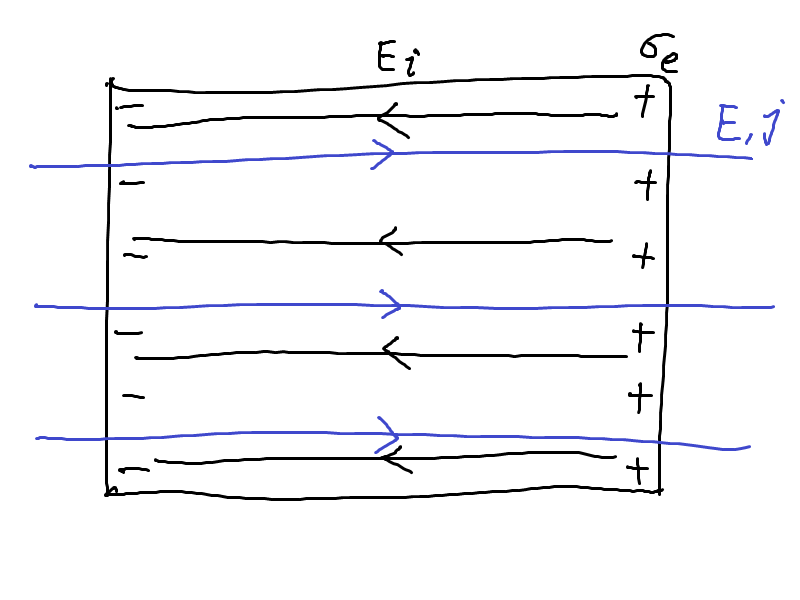
\includegraphics[scale=0.5]{fig/elec-equi}
\caption{吓得电荷都流过去了}
\label{fig-elec-equi}
\end{figure}

(高中学过的欧姆定律是$I=\frac{U}{R}$,而且$j=\frac{I}{S}$,$E=\frac{U}{l}$,$\rho=\frac{R S}{l}$,所以$j=\frac{E}{\rho}$,这是欧姆定律的微分形式)

导体的两边会积累电荷,电荷与电流的关系满足$\nabla \cdot \mathbf{j}=-\frac{\partial \rho_e}{\partial t}$,$\rho_e$是电荷密度。这就是电荷守恒定律的微分形式,表示某个点增加的电荷是从附近的电流流进来的。(你仍然可以检验一下两边量纲一样)

在导体的边界上,先看正电荷积累的一边,内侧有$j$流进去,而外侧没有,所以要把上面的方程改成$-j=-\frac{\opd \sigma_e}{\opd t}$,$\sigma_e$是电荷面密度。而负电荷积累的一边,内侧有$j$流出来,方程改成$j=-\frac{\opd (-\sigma_e)}{\opd t}$,跟正电荷那边一样。

这些电荷会产生反向的电场$E_i$,相当于一个平行板电容器,$E_i=\frac{\sigma_e}{\epsilon_0}$。

(高中学过电容器公式$C=\frac{S}{4 \pi k l}$,而且$\epsilon_0=\frac{1}{4 \pi k}$,$U=\frac{Q}{C}$,$E_i=\frac{U}{l}$,$\sigma_e=\frac{Q}{S}$,所以$E_i=\frac{\sigma_e}{\epsilon_0}$)

$E$和$E_i$都对电流有影响,刚才$j$的方程要改成$j=\frac{1}{\rho}(E-E_i)$。把上面的方程联立起来,得到$\sigma_e$满足的微分方程
\begin{equation*}
\frac{E}{\rho}-\frac{\sigma_e}{\epsilon_0 \rho}=\frac{\opd \sigma_e}{\opd t}
\end{equation*}

(如果你已经背出了它的解,可以跳过接下来的过程)令$x=\frac{E}{\rho}-\frac{\sigma_e}{\epsilon_0 \rho}$,$\opd x=-\frac{1}{\epsilon_0 \rho} \opd \sigma_e$,方程就变成了$x=-\epsilon_0 \rho \frac{\opd x}{\opd t}$,解得$x=x_0 \rme^{-\frac{t}{\epsilon_0 \rho}}$。

$t=0$时,$\sigma_e=0$,$x_0=\frac{E}{\rho}$,也就是$\frac{E}{\rho}-\frac{\sigma_e}{\epsilon_0 \rho}=\frac{E}{\rho} \rme^{-\frac{t}{\epsilon_0 \rho}}$,两边的电荷面密度$\sigma_e=\epsilon_0 E (1-\rme^{-\frac{t}{\epsilon_0 \rho}})$,总电场$E_s=E-E_i=E \rme^{-\frac{t}{\epsilon_0 \rho}}$。

可以看出,$t$很大时,$\sigma_e=\epsilon_0 E$,$E-E_i=0$,导体内没有电场。从数学上看,在有限的时间内,总电场只能无限接近零,而不可能严格为零。但是在一定的误差范围内,我们可以说它为零。

$\epsilon_0 \rho$的量纲是时间,所以把它称为特征时间$\tau$。每经过时间$\tau$,总电场就减小为$\frac{1}{e}$。

铜的电阻率$\rho=2 \times 10^{-8} \unit{\Omega \cdot m}$,所以$\tau=2 \times 10^{-19} \unit{s}$,电荷会迅速达到平衡。其他导体的$\tau$也差不多。
\section{磁单极子}
(这些东西只是为了好看放在这里)

假设磁单极子存在,用$q_m$表示它的磁荷。与电荷类比,它受到的洛伦兹力应该是$\mathbf{F}=q_m(\mathbf{B}-\frac{1}{c^2} \mathbf{v} \times \mathbf{E})$。$\frac{1}{c^2}$是为了凑量纲加上去的,负号则是为了让这个公式在洛伦兹变换下不变。可以看出,$q_m$的量纲是$[I] [T]$。

现在的麦克斯韦方程组是:
\begin{align*}
\nabla \cdot \mathbf{E}&=\frac{\rho_e}{\epsilon_0} & \nabla \cdot \mathbf{B}&=\mu_0 \rho_m \\
\nabla \times \mathbf{E}&=-\frac{1}{c^2} \frac{\mathbf{j}_m}{\epsilon_0}-\frac{\partial \mathbf{B}}{\partial t} & \nabla \times \mathbf{B}&=\mu_0 \mathbf{j}_e+\frac{1}{c^2} \frac{\partial \mathbf{E}}{\partial t}
\end{align*}

这样看起来就更有对称性了。正是从对称性考虑,许多理论都认为磁单极子应该存在,但是目前还没有实验能证明它存在。

(接下来我也不知道该讲什么了,可能要讲泊松方程和球坐标系下的分离变量,以及电磁场的能量、动量和角动量,还有辐射和天线的事情)
